% COS10022 Assignment 1 -- report guide (study notes, NOT report text)
\documentclass[11pt,a4paper]{article}
\usepackage[margin=2.2cm]{geometry}
\usepackage[T1]{fontenc}
\usepackage{lmodern}
\usepackage{amsmath}
\usepackage{booktabs,tabularx,array}
\usepackage{enumitem}
\usepackage[dvipsnames]{xcolor}
\usepackage[most]{tcolorbox}
\usepackage{pgfplots}
\pgfplotsset{compat=1.18}
\usepackage[hidelinks]{hyperref}
\setlist{itemsep=2pt,topsep=3pt}
\setlength{\parindent}{0pt}
\setlength{\parskip}{5pt}

\newtcolorbox{rubric}[1]{colback=Blue!4,colframe=Blue!60!black,fonttitle=\bfseries,title={#1},breakable}
\newtcolorbox{facts}{colback=Green!5,colframe=Green!50!black,fonttitle=\bfseries,title={Facts from the data (check them in your own KNIME run)},breakable}
\newtcolorbox{warn}{colback=Red!4,colframe=Red!60!black,fonttitle=\bfseries,title={Trap},breakable}
\newcommand{\node}[1]{\textsf{#1}}

\title{COS10022 Assignment 1 --- Report Guide\\[2pt]\large What theory and content your report needs}
\author{Study notes generated with Claude --- do not paste into your report}
\date{}

\begin{document}
\maketitle

\section*{How to use this guide}
This is a checklist of what each part of the report must contain, plus the theory behind it.
It is written as notes \emph{to you}. Write the report yourself, in your own words, from your
own KNIME run, in \texttt{report\_template.tex}. Declare any genAI use (including this guide) in
the appendix. The week~1 slides require prompts and outputs to be acknowledged.

\begin{rubric}{Hard requirements from the brief}
\begin{itemize}
  \item First page top: name, student ID, unit code, class (CL1/0x), tutor's name.
  \item At most 10 pages; mostly typed text (not screenshots of text); no table of contents needed.
  \item Answer the questions \emph{in the order of the brief}: Task~1 then Task~2.
  \item Turnitin below 25\% overall and below 5\% from any single source.
  \item Zip: workflow + input files in the workflow directory + output/intermediate files + video.
        The workflow must run and give the same numbers as the report.
\end{itemize}
\end{rubric}

\subsection*{Suggested page budget (10 pages max)}
\begin{tabularx}{\linewidth}{@{}Xr@{}}
\toprule
Section & Pages \\ \midrule
Introduction + dataset overview (short) & 0.5 \\
Task 1: workflow, node configuration, loading issues, results & 2.5 \\
Task 2: input, splitter, Workflow Coach, partitioning, models & 3.5 \\
Task 2: results, comparison, insights, suggestions & 2 \\
Exploration / reflection + conclusion & 1 \\
Appendix: genAI declaration (may sit after the 10 pages if your tutor allows; ask) & --- \\
\bottomrule
\end{tabularx}

%======================================================================
\section{Theory you need to understand}

\subsection{Where this sits in the Data Analytics Lifecycle}
The assignment covers Phase~3 (Model Planning: choosing LR, NB, RF) and Phase~4 (Model Building:
training on one dataset, evaluating on a separate test dataset). The lectures stress
\emph{documenting every decision} in Phase~4. That is the reason the rubric gives 15\% to node
configuration.

\subsection{Supervised classification}
Inputs: Age, Gender, Speed\_of\_Impact, Helmet\_Used, Seatbelt\_Used. Output (class label):
Survived = Yes/No. The training set teaches the model; the test set estimates performance on
unseen data. The lectures say training and test sets should be \emph{independent and
non-overlapping}. Keep that sentence in mind for the leakage discussion in Task~2.

\subsection{Logistic Regression}
A linear combination of the inputs, $z = w_0 + w_1x_1 + \dots + w_kx_k$, is passed through the
sigmoid:
\[
P(\text{Survived}=\text{Yes}\mid x) \;=\; \sigma(z) \;=\; \frac{1}{1+e^{-z}}
\]
\begin{center}
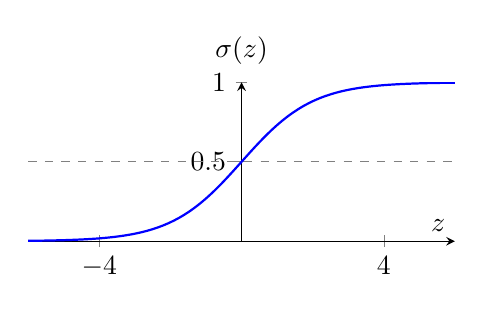
\begin{tikzpicture}
\begin{axis}[width=7cm,height=3.6cm,xmin=-6,xmax=6,ymin=0,ymax=1,
  axis lines=middle,xlabel={$z$},ylabel={$\sigma(z)$},ytick={0,0.5,1},xtick={-4,0,4},
  every axis y label/.style={at={(ticklabel* cs:1.05)},anchor=south}]
\addplot[domain=-6:6,samples=80,thick,Blue]{1/(1+exp(-x))};
\addplot[dashed,gray] coordinates {(-6,0.5) (6,0.5)};
\end{axis}
\end{tikzpicture}
\end{center}
\begin{itemize}
  \item The output is a probability in (0,1). Predict ``Yes'' if it is above the threshold (0.5 by default).
  \item Equivalently, $\log\frac{p}{1-p} = z$: each coefficient is the change in the \emph{log-odds}
        for a one-unit increase in that input. $e^{w}$ is the odds ratio.
  \item Nominal inputs (Gender, Helmet, Seatbelt) are dummy-coded; the coefficient is relative to the
        base level.
  \item \textbf{Reference category} (KNIME setting): coefficients describe the non-reference class
        against the reference. With reference = No, a positive coefficient means ``raises the odds of
        surviving''. State which reference you used, or readers can't interpret your signs.
  \item \textbf{Solver} (KNIME setting): IRLS (iteratively reweighted least squares) gives the exact
        maximum-likelihood solution and is deterministic. SAG (stochastic average gradient) is
        approximate, depends on epochs, step size and seed, and suits big data. Be able to justify your choice.
  \item The decision boundary is linear in the inputs. It cannot represent a sharp cut-off such as
        ``speed $\geq 90 \Rightarrow$ always dies'' except as a smooth slope. Expect this to limit LR.
\end{itemize}

\subsection{Naïve Bayes}
\[
P(c \mid a_1,\dots,a_m) \;\propto\; P(c)\prod_{j=1}^{m} P(a_j \mid c)
\]
\begin{itemize}
  \item ``Naïve'' = assumes the attributes are independent given the class.
  \item Nominal attributes: frequency tables. Numeric attributes (Age, Speed): KNIME fits a Gaussian per class.
        A Gaussian is a poor fit for a hard threshold at speed 90. Worth mentioning.
  \item $P(c)$ is the \textbf{prior}, learned from the class proportions in the training set. Your training
        set is 50/50 by construction, but the test set is about 94/6. The model's prior is therefore wrong
        for the test data, so it over-predicts ``Yes''. This is a strong insight point.
  \item Lecture advantages: simple, fast, needs little data. Disadvantage: the independence assumption.
\end{itemize}

\subsection{Random Forest}
\begin{itemize}
  \item An ensemble of decision trees. Each tree is trained on a \emph{bootstrap sample} (rows drawn
        with replacement) and considers a random subset of attributes at each split ($\sqrt{k}$ by default).
        The final prediction is the majority vote.
  \item Trees split on thresholds, so they can learn ``speed $\geq$ 90'' directly. That is
        non-linear behaviour LR can't express.
  \item Deep, unpruned trees can \emph{memorise} individual records. When test records also appear in the
        training data (see leakage below), RF benefits the most.
  \item Its result depends on a random seed. Fix it for reproducibility.
\end{itemize}

\subsection{Evaluation metrics (week 4 lecture)}
Confusion matrix with positive class = Yes:\quad
\begin{tabular}{@{}lcc@{}}\toprule & Pred.\ Yes & Pred.\ No\\\midrule Actual Yes & TP & FN\\ Actual No & FP & TN\\\bottomrule\end{tabular}
\begin{align*}
\text{Accuracy} &= \tfrac{TP+TN}{TP+TN+FP+FN} &
\text{Recall (TPR, sensitivity)} &= \tfrac{TP}{TP+FN} &
\text{Precision} &= \tfrac{TP}{TP+FP}\\
\text{Specificity (TNR)} &= \tfrac{TN}{TN+FP} &
F_1 &= \tfrac{2\cdot P \cdot R}{P+R} &
\text{Cohen's }\kappa &= \tfrac{p_o - p_e}{1-p_e}
\end{align*}
\begin{itemize}
  \item KNIME's Scorer shows all of these per class (Accuracy statistics port) plus Cohen's kappa.
  \item \textbf{Always compare against the majority-class baseline}: a model that always says ``No''.
        If the baseline is 94\%, an 85\% model is \emph{worse at accuracy} than doing nothing, even if
        it finds survivors. This is the core of the imbalance discussion.
  \item The lecture says a good model has accuracy of 80\% or more, \emph{but accuracy alone is not
        enough}. Use that line to motivate recall, precision and kappa.
\end{itemize}

\subsection{IID, sampling, reproducibility, leakage}
\begin{itemize}
  \item \textbf{IID} = independent and identically distributed: each record is drawn independently
        from the same distribution. The brief calls the balanced 700 set ``IID''. Think critically: a
        set with 50/50 classes no longer has the class distribution of the original data or of the
        test set. That is worth one or two sentences of reflection (rubric: critical thinking).
  \item \textbf{Random vs.\ top-k sampling}: the files are sorted, so ``take from top'' gives a biased sample.
  \item \textbf{Seeds}: Partitioning, Shuffle and RF are random. Without fixed seeds a re-run gives
        different numbers, and the brief says a mismatch with the report gets no mark.
  \item \textbf{Data leakage}: test records also present in the training set inflate test scores,
        because the model is partly ``tested'' on data it has already seen.
\end{itemize}

%======================================================================
\section{Dataset facts}
\begin{facts}
\begin{itemize}
  \item 6 columns: Age (int, 18--69), Gender (Male/Female), Speed\_of\_Impact (int, 20--119),
        Helmet\_Used (Yes/No), Seatbelt\_Used (Yes/No), Survived (Yes/No). No missing values.
  \item train1/train2: 420 rows each; test1/test2 (.csv): 180 rows each; test2.txt = test2.csv but
        \textbf{tab-separated with CRLF line endings}.
  \item train1+test1 and train2+test2 are \textbf{two different 70/30 splits of the same 600 records}.
        Reading all four CSVs gives 1,200 rows with every record twice (599 distinct).
  \item Files are sorted: all ``No'' rows first, then ``Yes'', each in descending speed.
  \item All 4 CSVs: 378 Yes / 822 No. After the split: train 350 Yes + 350 No = 700; test 28 Yes + 472 No = 500.
  \item Speed $\geq$ 90: survival 0\%. Speed $<$ 90: roughly 45\% survive. Age has almost no effect.
        Helmet and seatbelt raise survival. You can show this in KNIME with a GroupBy or chart:
        that counts as exploration.
\end{itemize}
\end{facts}

%======================================================================
\section{Task 1 --- what your section must contain}
\textit{Brief: explain how you came up with the workflow, the detailed configurations and why;
describe your prediction results; describe difficulties loading the files and how you solved them.}

\begin{rubric}{Rubric hooks: Workflow design 5\%, Node configuration 15\%, Data loading 10\%, Evaluation 10\%, Troubleshooting 5\%}
\begin{enumerate}
  \item \textbf{Workflow overview}: one screenshot of the Task~1 part, then 3--5 sentences on the logic
        (read train, read test, learn, predict, score) and \emph{why} the order matters.
  \item \textbf{Node configuration table}: one row per node with setting, value and \emph{justification}.
        Justification is what earns the 15\%. Include at least:
  \begin{itemize}
    \item CSV Reader (train): file, delimiter, header row, detected column types.
    \item CSV Reader (test): delimiter = Tab, and why.
    \item LR Learner: target column, included features, reference category, solver, max epochs/epsilon.
    \item LR Predictor: whether probabilities are appended.
    \item Scorer: actual vs.\ predicted column.
  \end{itemize}
  \item \textbf{Loading difficulty}: what you saw (the .txt read as one column), why (tab delimiter,
        CRLF), how you fixed it, how you confirmed the fix (6 columns, 180 rows, types match the
        training file). Screenshot before and after. Also mention that train and test must have
        identical column names and types for the predictor to work.
  \item \textbf{Results}: confusion matrix screenshot and accuracy statistics. Then interpret:
  \begin{itemize}
    \item accuracy compared with the always-``No'' baseline for this test set (111/180 = 61.7\%);
    \item recall for ``Yes'' (how many survivors it finds) compared with recall for ``No'';
    \item the coefficient table: which features increase or decrease survival odds, which are
          significant (p-value), and whether that makes sense (seatbelt, helmet, speed, age).
  \end{itemize}
\end{enumerate}
\end{rubric}
\begin{warn}
Expected Task~1 accuracy with IRLS: 64.4\% (No: 92 right/19 wrong; Yes: 45 wrong/24 right).
If yours differs a lot, check the delimiter and column types before writing anything.
\end{warn}

%======================================================================
\section{Task 2 --- what your section must contain}
\textit{Brief: how you took in all CSV files; the rules in the splitter; the prompt used to find the
partitioning node; detailed configuration of the data-preparation nodes; issues during training and
solutions; compare the three models; insights and suggestions.}

\subsection{Data preparation}
\begin{rubric}{Rubric hooks: Rule-based Row Splitter 5\%, Partitioning 10\%, Workflow Coach 5\%, Node configuration 15\%}
\begin{itemize}
  \item \textbf{Reading all CSVs}: CSV Reader in \emph{Files in folder} mode on \texttt{src}, with an
        extension filter for \texttt{csv}. Explain why: the brief forbids changing the src folder, and the
        .txt must be excluded. Mention the options you checked: RowID handling across files, and
        \emph{not} appending a path column (it would become a meaningless feature). Report the row
        count (1,200).
  \item \textbf{Splitter rule}: the exact rule text, which port holds which class, and the counts
        (378/822). Explain the rule syntax (\texttt{\$column\$}, \texttt{=>}, TRUE/FALSE).
  \item \textbf{Workflow Coach}: the \emph{exact prompt you typed}, a screenshot, which nodes it
        suggested, and why you picked Partitioning. Relate the prompt to the week~2 prompt structure
        (task, context, constraints). Write and try your own prompt; that is what is graded.
  \item \textbf{Partitioning (both)}: Absolute 350, Draw randomly, seed, and why ``random''
        (sorted files) and why a seed (reproducibility). Counts: 350/28 and 350/472.
  \item \textbf{Concatenate (both)}: which ports feed which node; how duplicate RowIDs are handled;
        result 700 and 500.
  \item \textbf{Shuffle (both)}: why shuffle (order-dependent learners, removes the class-sorted
        order), seed.
\end{itemize}
\end{rubric}

\subsection{Models}
\begin{rubric}{Rubric hooks: Model construction 5\%, Troubleshooting 5\%}
\begin{itemize}
  \item One configuration table per model (or one combined table): target, features, key parameters,
        seed, with justification. Confirm all three use the \emph{same} shuffled train and test nodes.
  \item Issues during training: report \emph{what actually happened to you} (error or warning text,
        cause, fix). Common ones: target column not nominal or not selected, a predictor fed the wrong
        port, Scorer comparing the wrong columns, results changing on every run (no seed), the NB
        nominal-values limit.
\end{itemize}
\end{rubric}

\subsection{Results, comparison, insights}
\begin{rubric}{Rubric hooks: Evaluation 10\%, Comparison \& insights 10\%}
\begin{enumerate}
  \item One comparison table: accuracy, Cohen's $\kappa$, recall/precision/F$_1$ for ``Yes'', recall for
        ``No'', for LR, NB and RF. Add the always-``No'' baseline (472/500 = 94.4\%) as its own row.
  \item Confusion-matrix screenshots for all three.
  \item Points to discuss (use your own numbers):
  \begin{itemize}
    \item \textbf{Imbalance}: all three models sit below the 94.4\% baseline on accuracy but find most
          of the 28 survivors. Discuss which metric matters for this problem, e.g.\ the cost of
          predicting ``survives'' for someone who won't (lecture: Type I vs.\ Type II error).
    \item \textbf{Prior shift}: trained on 50/50, tested on 94/6, so the models over-predict ``Yes''
          (low precision). NB is affected directly through $P(c)$.
    \item \textbf{Leakage}: about 44\% of test rows are identical to training rows (every record appears
          twice in the 4 CSVs). In the reference run RF scored 0.79 on those rows and 0.72 on unseen
          ones, while LR and NB showed no gap. Leakage favours the model that can memorise, but
          measure the size of the effect in your own run rather than assuming it. You can show
          this in KNIME (e.g.\ a Joiner between test and train, or a Duplicate Row Filter run).
    \item \textbf{Model behaviour}: RF can learn the speed-90 threshold; LR fits a smooth slope; NB's
          Gaussian and independence assumptions don't match that shape.
    \item Compare Task~1 LR with Task~2 LR, and explain why the numbers differ (different training
          distribution and test set).
  \end{itemize}
  \item \textbf{Suggestions}: remove duplicates (Duplicate Row Filter) before splitting; use stratified
        sampling or k-fold cross-validation (X-Partitioner/X-Aggregator, lecture week~4); evaluate with
        kappa, F$_1$ or AUC instead of accuracy; tune the decision threshold; collect more informative
        features.
\end{enumerate}
\end{rubric}

%======================================================================
\section{Exploration \& self-learning (10\%) and reflection}
Pick one or two small experiments and \emph{run them yourself}. Report what you expected, what
happened and what you learned:
\begin{itemize}
  \item Re-run Task~2 after a Duplicate Row Filter: how much do the RF numbers drop?
  \item LR solver: IRLS vs.\ SAG. Do the coefficients and accuracy change, and why?
  \item Change the seed 2--3 times: how stable are the results? That shows the variance of a single holdout split.
  \item Explore the speed threshold with a chart, linking data understanding to model choice.
\end{itemize}
The reflection should be specific: what surprised you, what you would do differently, how the
theory (prior, leakage, imbalance) explained something you saw.

%======================================================================
\section{Report quality (10\%)}
\begin{itemize}
  \item Number and caption every figure and table, and refer to each in the text (``Figure 3 shows~\dots'').
  \item Screenshots must be readable: crop to the relevant node or dialog.
  \item Use short paragraphs, consistent terms (``training set'', not three different names), and a
        spell check (genAI grammar help is an allowed use if declared).
  \item Cite the lecture or textbook (Dietrich 2015, EMC) when you state theory, so the theory is
        attributed and not copied.
\end{itemize}

\section{GenAI appendix}
List each tool, what you used it for, the prompts and the outputs (or excerpts), and what you changed
or verified yourself. Include: the KNIME Workflow Coach/K-AI prompts (part of the task), any use of
this guide or the reference workflow, and any grammar help.

\section{Video checklist}
Chain of thought (how you planned the workflow), the challenges (delimiter, reading the folder, exact
350 split, reproducibility, leakage) and how you solved them, and your takeaways. Show the workflow
running. Talk from your own understanding; the report and video should tell the same story.

\end{document}
